
%%%%%%%%%%%%%%%%%%%%%%%%%%%%%%%%%%%%%%%%%%%%%%%%%%%%%%%%%%%%%%%%%%%%%%%%%%%%%%%%%%%%%%%%%%%%%%%%
% Wärmelehre                                   
%%%%%%%%%%%%%%%%%%%%%%%%%%%%%%%%%%%%%%%%%%%%%%%%%%%%%%%%%%%%%%%%%%%%%%%%%%%%%%%%%%%%%%%%%%%%%%%%
\newpage
\section{Wärmelehre}
	\subsection{Einführung Wärmelehre}
	\subsubsection{Definitionen der Wärmelehre}\label{DefinitionenDerWaermelehre}
		\begin{minipage}{18cm}
			\begin{itemize}
				\item \textbf{Wärme(-energie) $\boldsymbol{Q}$:} eine Form der Energie, welche dem Gesetz der Energieerhaltung unterliegt und welche aufgrund einer Temperaturdifferenz übertragen wird. Die Wärme fliesst stets von der höheren zur tieferen Temperatur. [$Q$] = Joule, Kalorie
				\item \textbf{Temperatur:} ein Mass für die Bewegungsenergie der Moleküle eines Körpers oder Fluids
				\item \textbf{Tripelpunkt:} Punkt, an welchem feste, flüssige und gasförmige Phasen im Gleichgewicht sind. Ist die Temperatur unter dem Tripelpunkt geht ein Stoff direkt vom festen in den gasförmigen Zustand über ohne flüssig zu werden. \label{Tripelpunkt}
				\item \textbf{Kritische Temperatur:} Temperatur, oberhalb welcher die Verflüssigung eines Gases auch bei noch so hohem Druck nicht mehr möglich ist \label{KritischTemperatur}
				\item \textbf{Siedepunkt:} Gleichgewichtstemperatur zwischen Wasser und Dampf bei einem Luftdruck von 101 325 Pa
				\item \textbf{Eispunkt:} Gleichgewichtstemperatur zwischen Eis und luftgesättigtem Wasser bei einem Luftdruck von 101 325 Pa
				\item \textbf{Stoffmenge $\boldsymbol{n}$:} quantitative Mengenangabe von Stoffen, basierend auf 12g C-12-Kohlenstoff. $n = 6.022 \cdot 10^{23}$ Moleküle; [$n$] = mol (SI-Einheit)
				\item \textbf{Avogadrokonstante $\boldsymbol{N_A}$:} Anzahl Atome/Moleküle, welche in der Stoffmenge von 1 Mol enthalten sind
				\item \textbf{Extensive Grössen:} hängen von der Substanzmenge ab (z.B. Volumen, Stoffmenge)
				\item \textbf{Intensive Grössen:} sind von der Substanzmenge unabhängig (z.B. Temperatur)
				\item \textbf{Spezifische Grössen:} sind extensive Grössen pro Stoffmenge (z.B. Volumen/mol)
				\item \textbf{Offenes System:} System mit Energie- und Materieaustausch
				\item \textbf{Geschlossenes System:} System mit Energie-, aber ohne Materieaustausch
				\item \textbf{Abgeschlossenes System:} System ohne Energie- und ohne Materieaustausch
				\item \textbf{Adiabatisch:} System mit Arbeitsaustausch (Zustandsänderung), aber ohne Wärme- und ohne Materieaustauch
				\item \textbf{Isobar:} konstanter Druck
				\item \textbf{Isochor:} konstantes Volumen
				\item \textbf{Isotherm:} konstante Temperatur
				\item \textbf{Homogenes System:} System, das an allen Stellen die gleichen Eigenschaften hat
				\item \textbf{Heterogenes System:} System, das aus Bereichen mit verschiedenen Eigenschaften besteht, wobei sich dies an Grenzflächen abrupt ändern.
				\item \textbf{Phase:} Phase ist ein physikalisch und chemisch homogener Bereich in einem heterogenen System
				\item  \textbf{Aggregatszustand:} Unterschiedliche Zustände eines Stoffes, die sich durch bloße Änderungen von Temperatur oder Druck ineinander umwandeln können.
				\item \textbf{Dispersion:} Eine aus zwei oder mehreren Phasen bestehende Mischung, bei der eine Substanz in einer anderen in feinster Form verteilt ist
			\end{itemize}
		\end{minipage}

	\subsubsection{Wärmeeinheiten}
		\begin{minipage}{14cm}
			\begin{tabular}{ p{4cm} | p{6cm} }
				$T_K = T_C + 273.15$
				& $T_K$ = Temperatur in K\\
				$T_F = T_C \cdot 1.8 + 32$
				& $T_F$ = Temperatur in $^\circ F$\\
				& $T_C$ = Temperatur in $^\circ C$
			\end{tabular} 
		\end{minipage}
	
	\subsection{Thermische Zustandsgleichungen}
	\subsubsection{Wärmeausdehnung}
		\begin{minipage}{14cm}
			\myparagraph{Längen-, Flächen und Volumenausdehnung}
			\newline
				\begin{tabular}{ p{1.5cm} p{4.5cm} | p{7.5cm} }
					Fest:
					& 1D: $\Delta l = \alpha \cdot l_0 \cdot \Delta T $
						& $\alpha$ = Längenausdehungskoeffizient in $\frac{1}{K}$\\
					& 2D: $\Delta A = 2\alpha \cdot A_0 \cdot \Delta T$
						& $\gamma$ = Volumenausdehungskoeffizient\\
						&& \quad \quad in $\frac{1}{K} \text{ (für isotrope Mat.)}$\\
					& 3D: $\Delta V = \underbrace{3\alpha}_{\gamma} \cdot V_0 \cdot \Delta T$
						& T = Temperatur in K\\
					Flüssig:
					& 3D: $\Delta V = \gamma \cdot V_0 \cdot \Delta T$\\
					Gasförmig:
						& 3D: $\Delta V = \gamma \cdot V_0 \cdot \Delta T$\\
				\end{tabular} 
		\end{minipage}
		\begin{minipage}{10cm}
			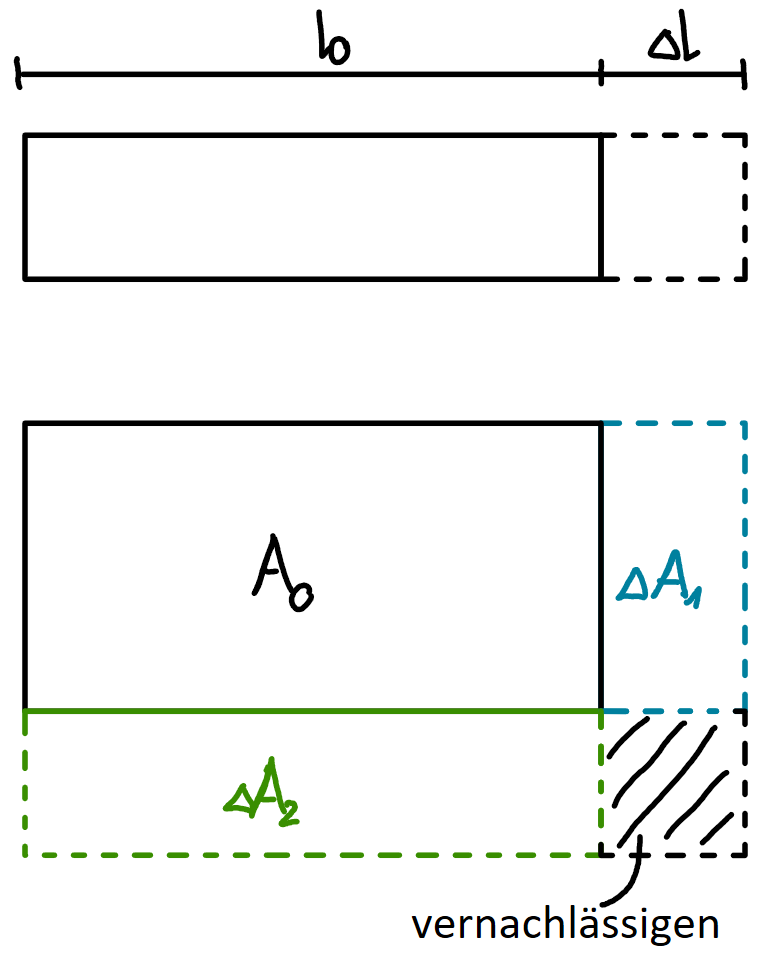
\includegraphics[width=3.5cm]{./bilder/Waermeausdehnung.png}
		\end{minipage}
		\begin{minipage}[t]{13cm}
			\myparagraph{Thermische Spannung (Hooksches Gesetz)}
			\begin{flushleft}
				Wird die thermische Ausdehnung behindert, treten mechanische Spannungen auf.
			\end{flushleft}
			\renewcommand{\arraystretch}{2.5}
			\begin{tabular}{ p{4cm} | p{7cm}}
				$\sigma = E \dfrac{\Delta l}{l_0} = E \alpha \Delta T$	&	$\sigma$ = thermische Spannung in $\frac{N}{m^2}$\\
			\end{tabular}
			\renewcommand{\arraystretch}{1.5}
			\begin{tabular}{ p{4cm} | p{7cm} }
				& $E$ = Elastizitätsmodul in $\frac{N}{m^2}$\\
				& $\alpha$ = Längenausdehnungskoeffizient in $\frac{1}{K}$\\
			\end{tabular} 
			\renewcommand{\arraystretch}{1}
		\end{minipage}

	\subsubsection{Ideale Gase}
		\begin{minipage}{15cm}
			\myparagraph{Eigenschaften idealer Gase}
				\begin{itemize}
					\item Die Moleküle sind Massenpunkte, d.h. sie haben eine Masse aber kein Volumen
					\item Es gibt keine intermolekularen Kräfte
					\item Die Gas-Temperatur ist weit höher als die kritische Temperatur
				\end{itemize}
				\renewcommand{\arraystretch}{1.5}
				\begin{tabular}{ | p{3cm} | p{4cm} | p{4cm} | p{4cm} |}
					\hline
					\textbf{Bezeichnung:} & \textbf{isobare} & \textbf{isochore} & \textbf{isotherme}\\
					\hline
				\end{tabular}
				\renewcommand{\arraystretch}{2}
				\begin{tabular}{ | p{3cm} | p{4cm} | p{4cm} | p{4cm} |}
					\textbf{Bedingung:} & p = konst & V = konst & T = konst\\
					\textbf{Formel:} & $\dfrac{V_1}{V_2} = \dfrac{T_1}{T_2}$ & $\dfrac{p_1}{p_2} = \dfrac{T_1}{T_2}$ & $\dfrac{p_1}{p_2} = \dfrac{V_2}{V_1}$\\
					\textbf{Gesetz:} & Gay-Lussac & Gay-Lussac & Boyle-Mariotte\\
					\hline
				\end{tabular}
				\renewcommand{\arraystretch}{1}
		\end{minipage}
		\newline
		\newline
		\newline
		\begin{minipage}{13cm}
			\myparagraph{Allgmeine Gasgleichung}
			\begin{flushleft}
				Avogadrosches Gesetz: Ideale Gase bei gleichem Druck und gleicher Temperatur enthalten in gleichen Volumina die gleiche Anzahl Moleküle.
			\end{flushleft}
			\renewcommand{\arraystretch}{2.5}
			\begin{tabular}{ p{5cm} | p{7cm}}
				$\dfrac{pV}{T} = konst$	&	$N$ = Anzahl Moleküle\\
				$pV = N k T = n \underbrace{N_A k}_R T = \dfrac{m}{M} R T$	&	$k$ = Boltzmann-Konstante = $1.381 \cdot 10^{-23} \frac{J}{K}$\\
			\end{tabular}
			\renewcommand{\arraystretch}{1.5}
			\begin{tabular}{ p{5cm} | p{7cm} }
				& $N_A$ = Avogadro-Konstante = $6.022 \cdot 10^{23}$\\
				& $n$ = Anzahl Mole\\
				& $R$ = Universelle Gaskonstante = $8.314 \frac{J}{mol \cdot K}$\\
				& $m$ = Masse vom Gas in $kg$\\
				& $M$ = Molmasse in $kg$\\
			\end{tabular} 
			\renewcommand{\arraystretch}{1}
		\end{minipage}
		\begin{minipage}{10cm}
			\vspace{-\ht\strutbox}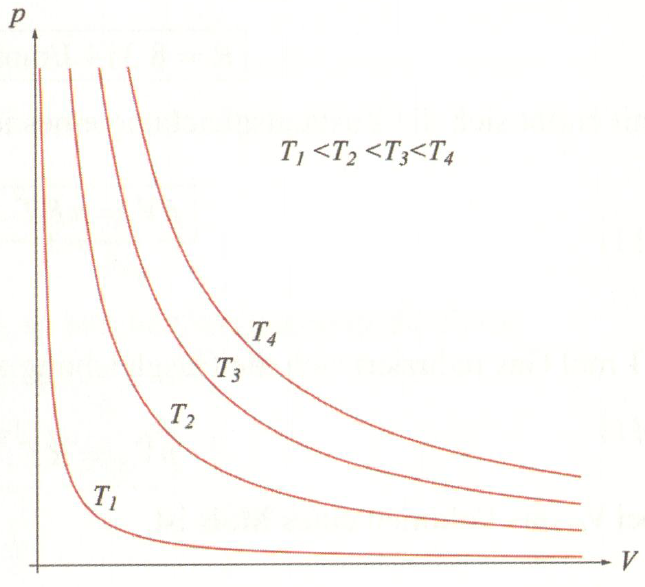
\includegraphics[width=6cm]{./bilder/Isotherme.png}
		\end{minipage}
		\newline
		\subsubsection{Gemische idealer Gase}
			\begin{minipage}[t]{10cm}
				\myparagraph{Gesetz von Dalton}
					\begin{flushleft}
						In einem Gasgemisch ist die Summe der Partialdrücke $p_i$ gleich dem Gesamtdruck $p$.
					\end{flushleft}
					\renewcommand{\arraystretch}{2.5}
					\begin{tabular}{ p{5cm} | p{7cm}}
						$p \cdot V = p(V_1 + V_2) = V(p_1 +p_2)$	&	$p_i$ = Partialdruck in $Pa$\\
						$p = \sum p_i$	& $p$ = Gesamtdruck in $Pa$\\
					\end{tabular}
					\renewcommand{\arraystretch}{1.5}
					\begin{tabular}{ p{5cm} | p{7cm}}
						& $V_i$ = Teilvolumen in $m^3$\\
						& $V$ = Gesamtvolumen in $m^3$\\
					\end{tabular} 
					\renewcommand{\arraystretch}{1}
			\end{minipage}
			\begin{minipage}[t]{10cm}
				\vspace{-\ht\strutbox}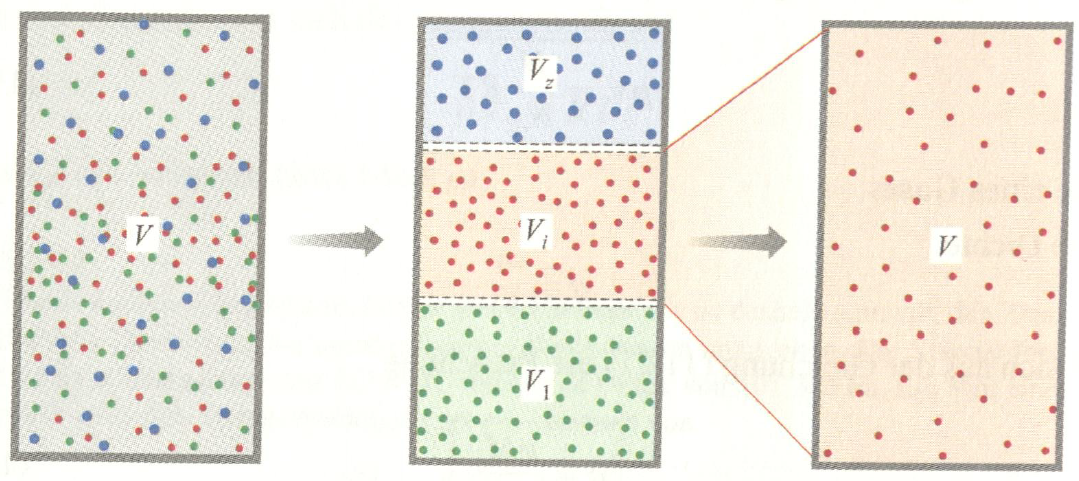
\includegraphics[width=9cm]{./bilder/GemischIdealerGase.png}
			\end{minipage}
		
	\subsubsection{Reale Gase}
		\begin{minipage}{15cm}
			\myparagraph{Eigenschaften realer Gase}
			\begin{itemize}
				\item Die Moleküle haben ein Eigenvolumen
				\item Es treten intermolekularen Kräfte auf
			\end{itemize}
		\end{minipage}
		\newline
		\newline
		\newline
		\newline
		\begin{minipage}{12.5cm}
			\myparagraph{Allgmeine Van der Waals'sche Zustandsgleichung}
				\newline
				\renewcommand{\arraystretch}{2.5}
				\begin{tabular}{ p{4cm} | p{7cm}}
					$p = \dfrac{nRT}{V-nb} - \dfrac{n^2 a}{V^2}$	&	$n$ = Anzahl Mole\\
				\end{tabular}
				\renewcommand{\arraystretch}{1.5}
				\begin{tabular}{ p{4cm} | p{7cm} }
					& $R$ = allgemeine Gaskonstante = $8.314 \frac{J}{mol \cdot K}$\\
					& $a, b$ = Van-der-Waals-Konstanten\\
				\end{tabular} 
				\renewcommand{\arraystretch}{1}
				\newline
				\newline
				\newline
				\textit{Achtung:} Das zwischen den Punkten A und D beschriebene Verhalten der Van der Waals'schen Zustandsgleichung ist unrealistisch. In der Realität bleibt der Druck zwischen den Punkten A und D konstant. Die Materie geht dabei vom gasförmigen in den flüssigen Zustand über.
		\end{minipage}
		\begin{minipage}{10cm}
			\vspace{-\ht\strutbox}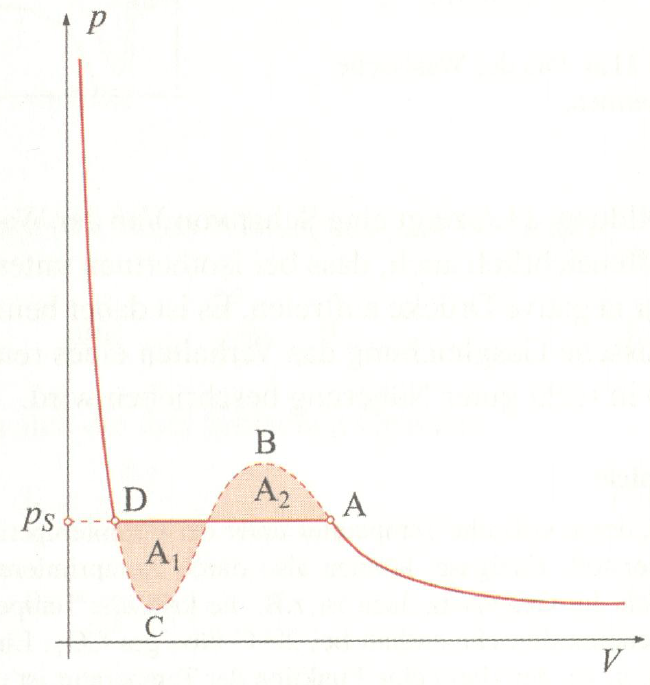
\includegraphics[width=6cm]{./bilder/VanDerWaalsscheZustandsfunktion.png}
		\end{minipage}
	\newpage
	\subsection{Kinetische Gastheorie}
		\begin{minipage}[t]{15cm}
			\subsubsection{Gasdruck}
				Die mittlere kinetische Energie der Moleküle ist proportional zur absoluten Temperatur.
				\newline
				\newline
				\renewcommand{\arraystretch}{2.5}
				\begin{tabular}{ p{4cm} | p{10cm}}
					$\overline{E_{kin}} = \dfrac{m\overline{v^2}}{2} = \dfrac{3}{2}kT$	&	$\overline{E_{kin}}$ = Mittlere kinetische Energie der Moleküle in $J$\\
				\end{tabular}
				\renewcommand{\arraystretch}{1.5}
				\begin{tabular}{ p{4cm} | p{7cm} }
					& $k$ = Boltzmannkonstannte =  $1.381 \cdot 10^{-23} \frac{J}{K}$\\
				\end{tabular} 
				\renewcommand{\arraystretch}{1}
		\end{minipage}
		\newline
		\newline
		\newline
		\newline
		\begin{minipage}[t]{10cm}
			\subsubsection{Äquipartiotionsgesetz}
				\renewcommand{\arraystretch}{2.5}
				\begin{tabular}{ p{2cm} | p{7cm}}
					$\overline{E} = \dfrac{f}{2}kT$	&	$\overline{E}$ = Gesamte mittlere Energie des Moleküls in $J$\\
				\end{tabular}
				\renewcommand{\arraystretch}{1.5}
				\begin{tabular}{ p{2cm} | p{7cm} }
					& $f$ = Anzahl Freiheitsgrade des Moleküls\\
					& $k$ = Boltzmannkonstannte =  $1.381 \cdot 10^{-23} \frac{J}{K}$\\
				\end{tabular} 
				\renewcommand{\arraystretch}{1}
		\end{minipage}
		\newline
		\newline
		\newline
		\newline
		\begin{minipage}[t]{18cm}
			\vspace{-\ht\strutbox}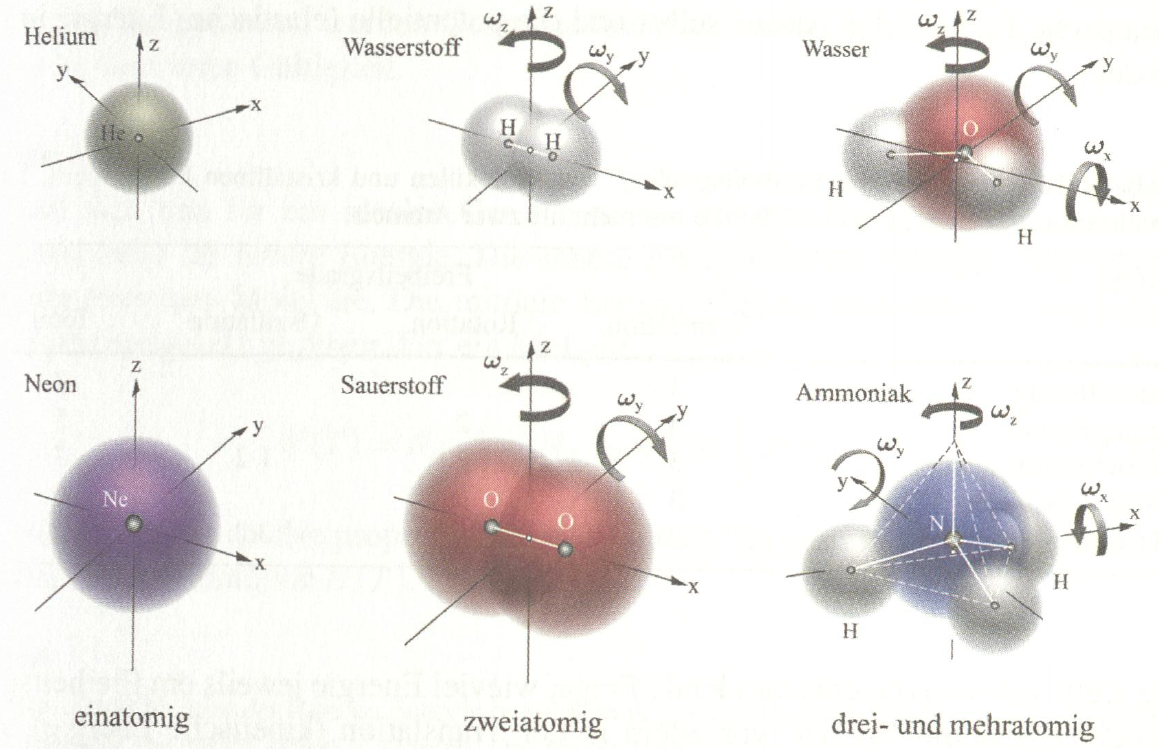
\includegraphics[width=10cm]{./bilder/FreiheitsgradeMolekuel.png}
		\end{minipage}
		\newline
		\newline
		\newline
		\newline
		\begin{minipage}{19cm}
			\renewcommand{\arraystretch}{1.5}
			\begin{tabular}{ | p{3cm} | p{13.28cm} |}
				\hline
				\textbf{Form:} & \textbf{Freiheitsgrade}\\
				\hline
			\end{tabular}
			\begin{tabular}{ | p{3cm} | p{3cm} | p{3cm} | p{3cm} | p{3cm} |}
				& Translation & Rotation & Oszillation & Total\\
				\hline
				Punktförmig & 3 & 0 & 0 & 3\\
				starre Hantel & 3 & 2 & 0 & 5\\
				schwingende Hantel & 3 & 2 & $1 \cdot 2$ & 7\\
				mehratomig starr & 3 & 3 & 0 & 6\\
				Kristall & 0 & 0 & $3 \cdot 2$ & 6\\
				\hline
			\end{tabular}
			\renewcommand{\arraystretch}{1}
			\vspace{3cm}
		\end{minipage}
		\newline
		\subsubsection{Maxwellsche Geschwindigkeitsverteilung}
		\begin{minipage}[t]{13cm}
			\myparagraph{Wahrscheinlichste Geschwindigkeit}
			\newline
			\renewcommand{\arraystretch}{2.5}
			\begin{tabular}{ p{3cm} | p{9cm}}
				$v_0 = \sqrt{\dfrac{2kT}{m}}$	&	$v_0$ = Wahrscheinlichste Geschwindigkeit in $\frac{m}{s}$\\
			\end{tabular}
			\renewcommand{\arraystretch}{1.5}
			\begin{tabular}{ p{3cm} | p{9cm} }
				& $k$ = Boltzmannkonstannte =  $1.381 \cdot 10^{-23} \frac{J}{K}$\\
			\end{tabular} 
			\renewcommand{\arraystretch}{1}
		\end{minipage}
		\newline
		\newline
		\newline
		\begin{minipage}[t]{13cm}
			\myparagraph{Mittlere Geschwindigkeit}
			\newline
			\renewcommand{\arraystretch}{2.5}
			\begin{tabular}{ p{3cm} | p{9cm}}
				$\overline{v} = \sqrt{\dfrac{8kT}{\pi m}}$	&	$\overline{v}$ = Mittlere Geschwindigkeit in $\frac{m}{s}$\\
			\end{tabular}
			\renewcommand{\arraystretch}{1.5}
			\begin{tabular}{ p{3cm} | p{9cm} }
				& $k$ = Boltzmannkonstannte =  $1.381 \cdot 10^{-23} \frac{J}{K}$\\
			\end{tabular} 
			\renewcommand{\arraystretch}{1}
		\end{minipage}
		\newline
		\newline
		\newline
		\begin{minipage}[t]{13cm}
			\myparagraph{Mittlere quadratische Geschwindigkeit}
			\newline
			\renewcommand{\arraystretch}{2.5}
			\begin{tabular}{ p{3cm} | p{9cm}}
				$u = \sqrt{\overline{v^2}}$ & $\overline{v}$ = Mittlere Geschwindigkeit in $\frac{m}{s}$\\
				$u = \sqrt{\dfrac{3kT}{m}}$	&	$u$ = mittlere quadratische Geschwindigkeit in $\frac{m}{s}$\\
			\end{tabular}
			\renewcommand{\arraystretch}{1.5}
			\begin{tabular}{ p{3cm} | p{9cm} }
				& $k$ = Boltzmannkonstannte =  $1.381 \cdot 10^{-23} \frac{J}{K}$\\
			\end{tabular} 
			\renewcommand{\arraystretch}{1}
		\end{minipage}
		\newline
		\newline
		\newline
		\subsubsection{Kinematik des Gases}
		\begin{minipage}[t]{13cm}
			\myparagraph{Mittlere freie Weglänge}
			\newline
			\renewcommand{\arraystretch}{2.5}
			\begin{tabular}{ p{3cm} | p{9cm}}
				$\overline{l} = \dfrac{1}{\sqrt{2}n\pi d^2}$	&	$l$ = mittlere freie Weglänge in $m$\\
			\end{tabular}
			\renewcommand{\arraystretch}{1.5}
			\begin{tabular}{ p{3cm} | p{9cm} }
				& $d$ = Molekül-Durchmesser in $m$\\
				& $n$ = Anzahl Moleküle pro Volumeneinheit\\
			\end{tabular} 
			\renewcommand{\arraystretch}{1}
		\end{minipage}
	
		\subsubsection{Transportvorgänge}
			\begin{minipage}{12cm}
				\myparagraph{Viskosität}
					\newline
					\renewcommand{\arraystretch}{2.5}
					\begin{tabular}{ p{4cm} | p{7cm}}
						$\eta = \dfrac{1}{3} \overline{v} \overline{l} \rho$	&	$\eta$ = Viskosität in $Pa \cdot s = \frac{N \cdot s}{m^2}$\\
					\end{tabular}
					\renewcommand{\arraystretch}{1.5}
					\begin{tabular}{ p{4cm} | p{10cm} }
						& $\overline{v}$ = Mittlere Geschwindigkeit in $\frac{m}{s}$\\
						& $\overline{l}$ = mittlere freie Weglänge in $m$\\
						& $\rho$ = Dichte Fluid in $\frac{kg}{m^3}$\\
					\end{tabular} 
					\renewcommand{\arraystretch}{1}
			\end{minipage}
	\newpage
	\subsection{Wärme}
		\begin{minipage}[t]{18cm}
			\subsubsection{Erster Hauptsatz der Thermodynamik}
				\begin{enumerate}
					\item  Die Innere Energie U ist die gesamte in einem System enthaltene Energie.
					\item Die Zunahme der inneren Energie eines thermodynamischen Systems ist gleich der Summe der von aussen zugeführten Arbeit und der von aussen zugeführt Wärme
				\end{enumerate}
				\renewcommand{\arraystretch}{2.5}
				\begin{tabular}{ p{4cm} | p{7cm}}
					$\mathrm{d} U = \delta W + \delta Q$	&	$U$ = Innere Energie in $J$\\
					$Q_{Ab} = Q_{Zu}$	& $W$ = Arbeit in $J$\\
				\end{tabular}
				\renewcommand{\arraystretch}{1.5}
				\newline
				\begin{tabular}{ p{4cm} | p{7cm} }
					& $Q$ = Wärme in $J$\\
					& $Q_{Ab}$ = Abgegebene Wärme in $J$\\
					& $Q_{Zu}$ = Zugeführte Wärme in $J$\\
				\end{tabular} 
				\renewcommand{\arraystretch}{1}
		\end{minipage}
		\newline
		\newline
		\newline
		\begin{minipage}[t]{18cm}
			\subsubsection{Spezifische und molare Wärmekapazität}
				\renewcommand{\arraystretch}{2.5}
				\begin{tabular}{ p{4cm} | p{7cm}}
					$c = \dfrac{C}{m}$	&	$c$ = spezifische Wärmekapazität in $\frac{J}{kg \cdot K}$\\
					$\delta Q = cm \mathrm{d} T$	&	$C$ = Wärmekapazität in $\frac{J}{K}$\\
					$C_m = \dfrac{c}{n} = \dfrac{MC}{m} = Mc$ & $C_m$ = molare Wärmekapazität in $\frac{J}{mol \cdot K}$
				\end{tabular}
				\renewcommand{\arraystretch}{1.5}
				\newline
				\begin{tabular}{ p{4cm} | p{7cm} }
					& $Q$ = Wärme in $J$\\
					& $n$ = Stoffmenge = Anzahl Mol\\
					& $M$ = Molmasse in $kg$\\
				\end{tabular} 
				\renewcommand{\arraystretch}{1}
		\end{minipage}
		\newline
		\newline
		\newline
		\begin{minipage}[t]{18cm}
			\subsubsection{Verbrennungsenergie}
				\renewcommand{\arraystretch}{2.5}
				\begin{tabular}{ p{4cm} | p{7cm}}
					$H_f = \dfrac{Q}{m}$	&	$H_f$ = Heizwert in $\frac{J}{kg}$\\
					$H_g = \dfrac{Q}{V}$	&	$H_G$ = Brennwert in $\frac{J}{m^3}$\\
				\end{tabular}
				\renewcommand{\arraystretch}{1.5}
				\newline
				\begin{tabular}{ p{4cm} | p{7cm} }
					& $Q$ = Wärme in $J$\\
				\end{tabular} 
				\renewcommand{\arraystretch}{1}
		\end{minipage}
	
	\newpage
	\subsection{Phasen und Phasenübergänge}
		\begin{minipage}[t]{13cm}
			\subsubsection{Phasenübergänge}
			\renewcommand{\arraystretch}{2.5}
			\begin{tabular}{ p{4cm} | p{7cm}}
				$q_f = \dfrac{Q_f}{m}$	&	$q_f$ = spezifische Schmelzwärme in $\frac{J}{kg}$\\
				$q_s = \dfrac{Q_s}{m}$	&	$q_s$ = spezifische Verdampfungswärme in $\frac{J}{kg}$\\
			\end{tabular}
			\renewcommand{\arraystretch}{1.5}
			\begin{tabular}{ p{4cm} | p{7cm} }
				& $Q_f$ = Schmelzwärme in $J$\\
				& $Q_s$ = Verdampfungswärme in $J$\\
			\end{tabular} 
			\renewcommand{\arraystretch}{1}
		\end{minipage}
		\newline
		\newline
		\subsubsection{Phasendiagramm}
		\begin{minipage}[t]{7cm}
			\vspace{-\ht\strutbox}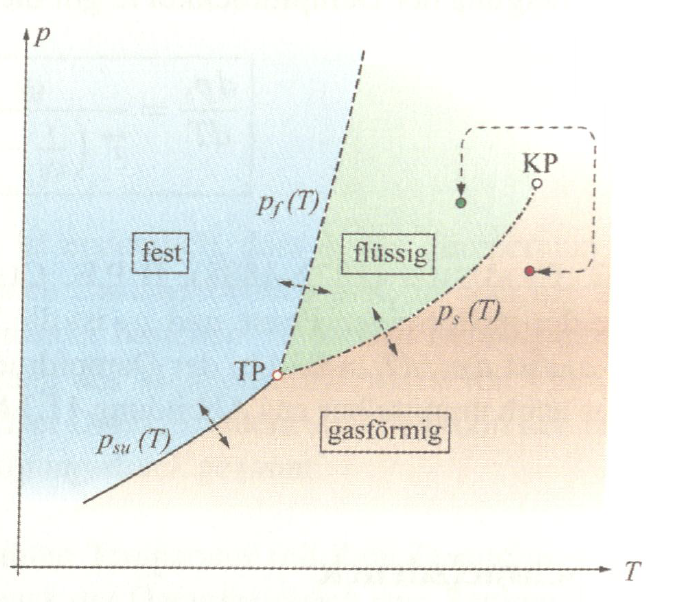
\includegraphics[width=7cm]{./bilder/Phasendiagramm.png}
		\end{minipage}
		\begin{minipage}[t][7cm][t]{10cm}
			\vspace{2.3cm}
			TP = Tripelpunkt\\
			KP = Krititische Temperatur\\ \\
			(für Begriffserklärung siehe Kap. \ref{DefinitionenDerWaermelehre} \nameref{DefinitionenDerWaermelehre})
		\end{minipage}
		\newline
		\subsubsection{Luftfeuchtigkeit}
			\begin{minipage}[t]{13cm}
				\myparagraph{Formeln von Magnus}
					\renewcommand{\arraystretch}{3}
					\begin{tabular}{ p{6.5cm} | p{9cm}}
						$\vartheta \geq 0 $\textdegree$ C$: \quad $p_s = p_{s0} \cdot 10^{\frac{7.5 \vartheta}{\vartheta +237}}$	&	$\vartheta$ = Temperatur in \textdegree $C$\\
						$\vartheta \leq 0 $\textdegree$ C$: \quad $p_s = p_{s0} \cdot 10^{\frac{9.5 \vartheta}{\vartheta +265.5}}$	&	$\vartheta_d$ = Taupunkts-Temperatur in \textdegree $C$\\
						$p_s \geq 6.107hPa$: \quad $\vartheta = \dfrac{237 \cdot \log{(\frac{p_s}{6.107})}}{7.5 - \log{(\frac{p_s}{6.107})}}$	&	$p_s$ = Sättigungsdruck in $hPa$\\
						$p_s \leq 6.107hPa$: \quad $\vartheta = \dfrac{265.5 \cdot \log{(\frac{p_s}{6.107}})}{9.5 - \log{(\frac{p_s}{6.107})}}$	&	$p_{s0}$ = Dampfdruck in $hPa$ $(= 6.107hPa$ bei $0 $\textdegree$ C)$\\
						$\vartheta_d = \dfrac{237 \cdot (\log{(f_r)} + \frac{7.5 \cdot \vartheta}{\vartheta +237})}{7.5 - (\log{(f_r)} + \frac{7.5 \cdot \vartheta}{\vartheta +237})}$	& $f_r$ = relative Luftfeuchtigkeit (dimensionslos)\\
					\end{tabular}
					\renewcommand{\arraystretch}{1}
			\end{minipage}

	\newpage
	\subsection{Wärmetransport}
		\subsubsection{Wärmeleitung}
			\begin{minipage}[t]{16cm}
				\myparagraph{Fouriersches Gesetz der Wärmeleitung (Stationär (Zeitunabhängig))}
					\renewcommand{\arraystretch}{2.5}
					\begin{tabular}{ p{4cm} | p{7cm}}
						$j = -\lambda \dfrac{\mathrm{d}T}{\mathrm{d}x}$	&	$j$ = Wärmestromdichte in $\frac{W}{m^2}$\\
					\end{tabular}
					\renewcommand{\arraystretch}{1.5}
					\begin{tabular}{ p{4cm} | p{7cm} }
						& $\lambda$ = Wärmeleitfähigkeit in $\frac{W}{m \cdot K}$\\
						& $x$ = Distanz in x-Richtung in $m$\\
					\end{tabular} 
					\renewcommand{\arraystretch}{1}
			\end{minipage}
		\newline
		\newline
		\begin{minipage}[t]{13cm}
			\subsubsection{Wärmeleitungsgleichung (Instationär (Zeitabhängig))}
				\renewcommand{\arraystretch}{2.5}
				\begin{tabular}{ p{4cm} | p{7cm}}
					$\dfrac{\partial T}{\partial t} = \underbrace{\dfrac{\lambda}{\rho c}}_a \cdot \dfrac{\partial^2 T}{\partial x^2}$	& $\lambda$ = Wärmeleitfähigkeit in $\frac{W}{m \cdot K}$\\
				\end{tabular}
				\renewcommand{\arraystretch}{1.5}
				\begin{tabular}{ p{4cm} | p{7cm} }
					& $x$ = Distanz in x-Richtung in $m$\\
					& $\rho$ = Materialdichte in $kg/m^3$\\
					& $c$ = spezifische Wärmekapazität in $\frac{J}{kg \cdot K}$\\
					& $a$ = Temperaturleitfähigkeit in $\frac{m^2}{s}$
				\end{tabular} 
				\renewcommand{\arraystretch}{1}
		\end{minipage}
		\newline
		\newline
		\begin{minipage}[t]{11.5cm}
			\subsubsection{Wärmeübergang}
				\renewcommand{\arraystretch}{2.5}
				\begin{tabular}{ p{4cm} | p{7cm}}
					$j = \alpha(T_w -T)$	&	$j$ = Wärmestromdichte in $\frac{W}{m^2}$\\
				\end{tabular}
				\renewcommand{\arraystretch}{1.5}
				\begin{tabular}{ p{4cm} | p{7cm} }
					& $\alpha$ = Wärmeübergangszahl in $\frac{W}{m^2 \cdot K}$\\
					& $T_w$ = Temperatur an der Wand in $K$\\
					& $T$ = Umgebungstemperatur in $K$\\
				\end{tabular} 
				\renewcommand{\arraystretch}{1}
		\end{minipage}
		\begin{minipage}[t]{10cm}
			\vspace{-\ht\strutbox}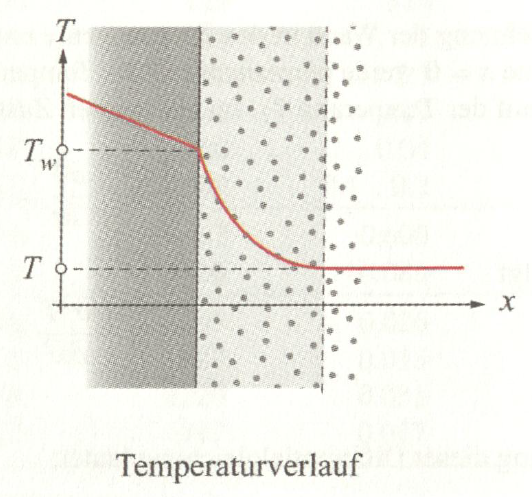
\includegraphics[width=5.5cm]{./bilder/Waermeuebergang.png}
		\end{minipage}
		\newline
		\newline
		\newline
		\newline
		\begin{minipage}{12cm}
			\myparagraph{Typische Wärmeübergangszahlen für Gebäude}
			\newline
			\renewcommand{\arraystretch}{1.5}
			\begin{tabular}{ | p{5cm} | p{3cm} |}
				\hline
				\textbf{an} & $\boldsymbol{\alpha}$ in $\frac{W}{m^2 \cdot K}$\\
				\hline
				Wandflächen & \\
				\quad innen & 8\\
				\quad aussen & 20\\
				\hline
				Böden und Decken & \\
				\quad Wärmestrom nach oben & 8\\
				\quad Wärmestrom nach unten & 6\\
				\hline
			\end{tabular}
			\renewcommand{\arraystretch}{1}
		\end{minipage}
		\vspace{3cm}
		\newline
		\subsubsection{Wärmedurchgang}
			\begin{minipage}{12cm}
				\myparagraph{Wärmedurchgang durch ebene (mehrschichtige) Wand}
					\renewcommand{\arraystretch}{2.5}
					\begin{tabular}{ p{4cm} | p{7cm}}
						$k = \dfrac{1}{\dfrac{1}{\alpha_i} + \sum\limits_{s}\dfrac{d_s}{\lambda_s} + \dfrac{1}{\alpha_a}}$	&	$k$ = k-Wert, Wärmedurchgangszahl in $\frac{W}{m^2 \cdot K}$\\
						$j = k \Delta T$	&	$\alpha_i$ = Wärmeübergangszahl innen in $\frac{W}{m^2 \cdot K}$\\
					\end{tabular}
					\renewcommand{\arraystretch}{1.5}
					\begin{tabular}{ p{4cm} | p{7cm} }
						& $\alpha_a$ = Wärmeübergangszahl aussen in $\frac{W}{m^2 \cdot K}$\\
						& $d_s$ = Wandstärke Schicht s in $m$\\
						& $\lambda_s$ = Wärmeleitfähigkeit Schicht s in $\frac{W}{m \cdot K}$\\
						& $j$ = Wärmestromdichte in $\frac{W}{m^2}$\\
					\end{tabular} 
					\renewcommand{\arraystretch}{1}
			\end{minipage}
			\begin{minipage}{10cm}
				\vspace{-\ht\strutbox}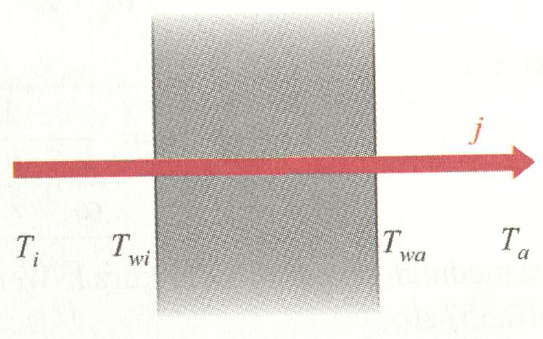
\includegraphics[width=6.5cm]{./bilder/Waermedurchgang.png}
			\end{minipage}
			\newline
			\newline
			\newline
			\newline
			\begin{minipage}{12cm}
				\myparagraph{Wärmedurchgang durch kreiszylindrische (mehrschichtige) Wand}
					\renewcommand{\arraystretch}{2.5}
					\begin{tabular}{ p{7cm} | p{7cm}}
						$k_a = \dfrac{1}{r_a} \cdot \dfrac{1}{\dfrac{1}{r_i \alpha_i} + \sum\limits_{s}\dfrac{1}{\lambda_s} \ln(\dfrac{r_{sa}}{r_{si}}) + \dfrac{1}{r_a \alpha_a}}$	&	$k_a$ = k-Wert, Wärmedurchgangszahl in $\frac{W}{m^2 \cdot K}$\\
					\end{tabular}
					\renewcommand{\arraystretch}{1.5}
					\begin{tabular}{ p{7cm} | p{7cm} }
						& $r_i$ = Innenradius in $m$\\
						& $r_a$ = Aussenradius in $m$\\
						& $r_{si}$ = Innenradius Schicht s in $m$\\
						& $r_{sa}$ = Aussenradius Schicht s in $m$\\
						& $\alpha_i$ = Wärmeübergangszahl innen in $\frac{W}{m^2 \cdot K}$\\
						& $\alpha_a$ = Wärmeübergangszahl aussen in $\frac{W}{m^2 \cdot K}$\\
						& $\lambda_s$ = Wärmeleitfähigkeit Schicht s in $\frac{W}{m \cdot K}$\\
					\end{tabular} 
					\renewcommand{\arraystretch}{1}
			\end{minipage}
			\newline
			\newline
			\newline
			\begin{minipage}[t]{13cm}
				\subsubsection{Wärmebedarf eines Gebäudes}
					\renewcommand{\arraystretch}{2.5}
					\begin{tabular}{ p{5cm} | p{13cm}}
						$Q_{tot} = Q_W + Q_L$	&	$Q_{tot}$ = totale Wärme in $J$\\
						$Q_W = Aj = Ak \Delta T$	&	$Q_W$ = Wärmefluss durch alle Wände in $J$\\
						$Q_L = c_l \cdot \rho_l \cdot \dfrac{V}{t} \Delta T $	&	$Q_L$ = Wärmefluss durch Lüftung in $J$\\
						$Q = (\sum\limits_{w} A_W k_W + \rho \cdot c_l \cdot \dfrac{V}{t}) G$ & $A$ = Wandfläche in $m^2$\\
					\end{tabular}
					\renewcommand{\arraystretch}{1.5}
					\begin{tabular}{ p{5cm} | p{13cm} }
						& $j$ = Wärmestromdichte in $\frac{W}{m^2}$\\
						& $k_a$ = k-Wert, Wärmedurchgangszahl in $\frac{W}{m^2 \cdot K}$\\
						& $c_l$ = spezifische Wärmekapazität in $\frac{J}{kg \cdot K}$\\
						& $\rho_l$ = Luftdichte in $\frac{kg}{m^3}$\\
						& $V$ = Raumvolumen in $m^3$\\
						& $t$ = Dauer des Luftwechsels in $s$ (Bsp. 2-facher Luftwechsel pro Stunde $= \frac{3600s}{2}$)\\
						& $G$ = Heizgradtage in $K \cdot d$ (=Kelvin mal Tage)\\
					\end{tabular} 
					\renewcommand{\arraystretch}{1}
			\end{minipage}
		
	\newpage
	\subsection{Zustandsänderungen}
		\subsubsection{Reversible und irreversible Prozesse}
			\begin{minipage}[t]{13cm}
				\myparagraph{Reversible Prozesse}
					\newline
					Ein reversibler Prozess kann umgekehrt durchlaufen werden, wobei der Ausgangszustand wieder erreicht wird, ohne dass in der Umgebung irgendwelche Änderung zurückbleiben.
			\end{minipage}
			\newline
			\newline
			\begin{minipage}[t]{13cm}
				\myparagraph{Irreversible Prozesse}
					\newline
					Ein irreversibler Prozess kann nicht umgekehrt durchlaufen werden, ohne dass in der Umgebung irgendwelche Änderungen zurückbleiben.
			\end{minipage}
	
	\vspace{2cm}
	\subsection{Kreisprozesse und Zweiter Hauptsatz}
		\subsubsection{Kreispprozess von Carnot}
			\begin{minipage}[t]{13cm}
				\myparagraph{Carnot-Wirkungsgrad (Wärmekraftmaschine)}
					\renewcommand{\arraystretch}{2.5}
					\begin{tabular}{ p{5cm} | p{9cm}}
						$\eta_C = \dfrac{T_1 - T_2}{T_1} < 1$	&	$\eta_C$ = Carnot-Wirkungsgrad (einheitslos)\\
					\end{tabular}
					\renewcommand{\arraystretch}{1}
					\newline
					\newline
				\myparagraph{Inverser Carnot-Wirkungsgrad (Wärmepumpe)}
					\renewcommand{\arraystretch}{2.5}
					\begin{tabular}{ p{5cm} | p{9cm}}
						$\eta_{iC} = \dfrac{1}{\eta_C} = \dfrac{T_1}{T_1 - T_2} > 1$	&	$\eta_{iC}$ = Inverser Carnot-Wirkungsgrad (einheitslos)\\
					\end{tabular}
					\renewcommand{\arraystretch}{1}
			\end{minipage}
			\newline
			\newline
			\newline
			\newline
			\begin{minipage}[t]{7cm}
				\vspace{-\ht\strutbox}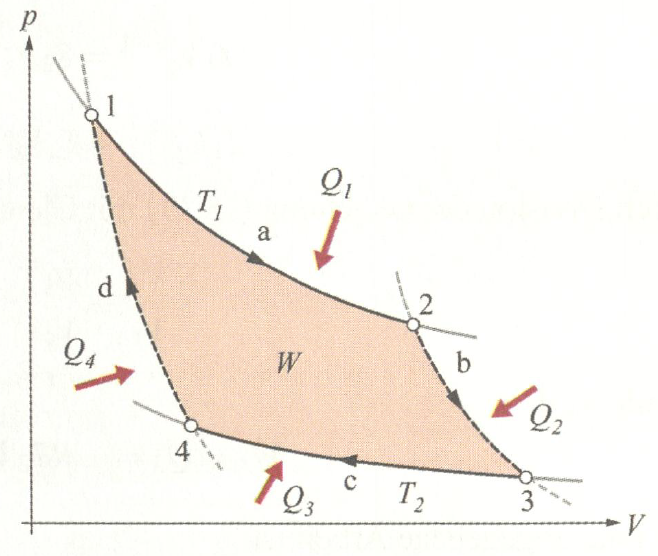
\includegraphics[width=7cm]{./bilder/KreisprozessCarnot.png}
			\end{minipage}
			\begin{minipage}[t]{10cm}
				\begin{enumerate}
					\vspace{1cm}
					\item isotheme Expansion bei der Temperatur $T_1$
					\item adiabatische Expansion
					\item isotherme Kompression bei der Temperatur $T_2$
					\item adiabatische Kompression
				\end{enumerate}
			\end{minipage}
		
